%Empieza configuracion de capitulo
\setstretch{1.0}
\titleformat{\chapter}[block]{\Large\bfseries}{CAP'ITULO \Huge\thechapter\vspace{25 pt}}{0 pt}{\\\fontsize{26}{36}\selectfont}
\titlespacing{\chapter}{0 pt}{30 pt}{50 pt}[0 pt]
\titleformat{\section}{\Large\bfseries}{\thesection}{0 pt}{\hspace{30 pt}}
\titleformat{\subsection}{\large\bfseries}{\thesubsection}{0 pt}{\hspace{30 pt}}
\pagestyle{fancy}
\fancyhead[LO,LE]{\footnotesize\textit{\leftmark}}
\fancyhead[RO,RE]{\thepage}
\fancyfoot[CO,CE]{}
%Termina configuracion de capitulo

\chapter{Desarrollo del Trabajo} %Cambia al nombre de tu capitulo
\setstretch{1.5} %Regresa el interlineado a 1.5

\normalsize

\section{Concepto de Operaciones}
\label{sec:ConceptoDeOperaciones}
\noindent
El BM es un sistema de administraci'on, de seguimiento y de mejora continua de la calidad personal y grupal en el desarrollo de sistemas de software. Esto lo realiza mediante el seguimiento de proyectos, seguimiento de actividades de desarrollo, seguimiento de actividades de calidad, administraci'on de defectos y generaci'on de estad'isticas y m'etricas verdaderamente 'utiles para las organizaciones de software.

El BM tiene la flexibilidad necesaria para que la persona responsable dentro de la organizaci'on defina el ciclo de vida y las actividades por realizar dentro de un proyecto de software. As'i mismo podr'a definir la taxonom'ia a utilizar respecto a los diferentes defectos dentro del sistema, as'i como las plantillas a utilizar para las actividades de calidad. Esta flexibilidad permitir'a que la aplicaci'on pueda ser adoptada por un gran n'umero de organizaciones de software con diferentes procesos de desarrollo de software.

El sistema estar'a basado en la tecnolog'ia web, por lo que no ser'a necesaria la instalaci'on f'isica de la aplicaci'on en los clientes que pretendan acceder a ella. S'olo ser'a necesario el uso del navegador para acceder a este sistema y la instalaci'on se har'a en el servidor dedicado a la aplicaci'on.

\subsection{Objetivos}
\noindent
Los objetivos principales del sistema son:

\begin{itemize}
	\item Lograr una mejora continua en el proceso de desarrollo de software, as'i como una mayor calidad en el producto final.
	\item Reducir el costo de implementar actividades de calidad dentro de la empresa.
	\item Proporcionar informaci'on valiosa a la empresa para la toma de decisiones respecto a cambios en sus procesos de desarrollo de software.
	\item Facilitar la evoluci'on y adaptaci'on de las diferentes actividades de aseguramiento de la calidad.
	\item Promover una cultura de calidad personal enfocada en la prevenci'on de defectos.
	\item Proveer datos sobre el esfuerzo (costo) de las actividades de remoci'on de defectos.
	\item Facilitar un cambio cultural respecto a la forma de trabajar de peque'nas y medianas empresas.
\end{itemize}

\subsection{Alcances}
\noindent
Se puede definir como alcance en cuanto a funcionalidad lo siguiente:

\begin{itemize}
	\item Registrar y dar seguimiento a las actividades de desarrollo y calidad establecidas para el ciclo de vida de desarrollo.
	\item Hacer un seguimiento puntual a la inyecci'on, remoci'on y correcci'on de defectos a lo largo de las diferentes etapas del ciclo de vida.
	\item Generar estad'isticas y m'etricas de valor para la empresa y el personal en base a la informaci'on proporcionada por los usuarios del sistema.
	\item Dar una gu'ia en los procedimientos principales de aseguramiento de la calidad.
\end{itemize}

\subsection{M'odulos del Sistema}
\noindent
El BM est'a dividido en 5 m'odulos representados en la figura \ref{fig:ModulosBM}:

\begin{itemize}
	\item \emph{M'odulo de Administraci'on}. Este m'odulo est'a encargado de realizar las altas, bajas y cambios de proyectos, actividades y usuarios.
	\item \emph{M'odulo de Actividades}. Este m'odulo est'a encargado de realizar la actualizaci'on de actividades y las tareas relacionadas con el seguimiento del proyecto.
	\item \emph{M'odulo de Calidad}. Este m'odulo est'a encargado de las plantillas para las actividades de remoci'on de defectos, as'i como el ciclo de vida para los proyectos.
	\item \emph{M'odulo de Defectos}. Este m'odulo est'a encargado del registro y seguimiento de defectos.
	\item \emph{M'odulo de Reportes}. Este m'odulo est'a encargado de la generaci'on de reportes estad'isticos personales, por proyecto, por equipo y de empresa.
\end{itemize}

\begin{figure}[h]
	\centering
		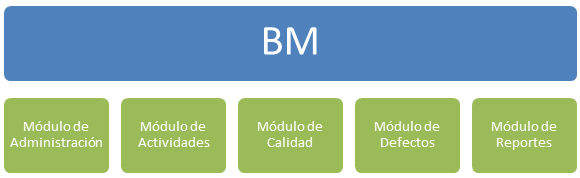
\includegraphics[scale=0.9]{images/ModulosBM.png}
	\caption{M'odulos del BM}
	\label{fig:ModulosBM}
\end{figure}

\subsection{Tipos de Usuario}
\noindent
El BM tendr'a tres tipos de usuarios: Administrador, L'ider de Proyecto y Usuario.  Est'an representados en la figura \ref{fig:UsuariosBM} que nos muestra los usuarios por nivel. Se representa en una pir'amide invertida para denotar los privilegios y que los niveles superiores tienen toda la funcionalidad de los niveles inferiores. Entonces el Administrador puede utilizar la funcionalidad del L'ider de Proyecto y del Usuario; mientras que el L'ider de Proyecto tiene acceso a la funcionalidad de Usuario.

\begin{figure}[h]
	\centering
		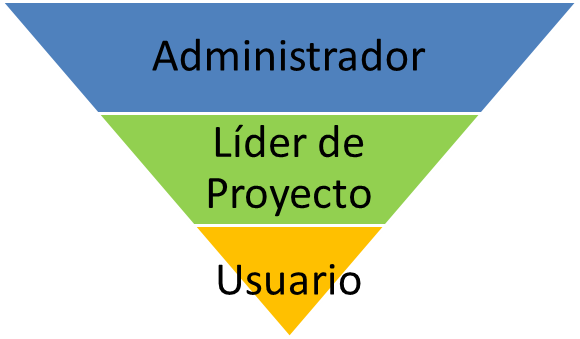
\includegraphics[scale=0.7]{images/UsuariosBM.png}
	\caption{Tipos de usuario del BM}
	\label{fig:UsuariosBM}
\end{figure}

Sus caracter'isticas y funcionalidades principales son: 

\begin{itemize}
	\item \emph{Administrador}. Es el tipo de usuario con m'as privilegios en el sistema y tiene responsabilidades y derechos a nivel organizaci'on, representa a la gerencia de la organizaci'on. Sus actividades principales son:
	\begin{itemize}
		\item Alta, baja y modificaci'on de proyectos.
		\item Alta, baja y modificaci'on de usuarios.
		\item Asignaci'on de recursos a proyectos.
		\item Revisi'on de reportes y m'etricas por organizaci'on, proyecto e individuales.
	\end{itemize}
	\item \emph{L'ider de Proyecto}. Es el tipo de usuario que le sigue en privilegios al Administrador y tiene responsabilidades y derechos a nivel de proyecto, representa al l'ider de uno o varios proyectos. Sus actividades principales son:
	\begin{itemize}
		\item Definici'on de tipos de defecto.
		\item Definici'on de ciclo de vida para el proyecto.
		\item Definici'on de plantillas p'ublicas para las actividades de calidad.
		\item Definici'on de actividades de desarrollo y de actividades de calidad.
		\item Asignaci'on de las actividades a los usuarios.
		\item Revisi'on de reportes y m'etricas a nivel proyecto e individuales.
	\end{itemize}
	\item \emph{Usuario}. Es el tipo de usuario con menos privilegios, representa un desarrollador del proyecto. Sus actividades principales son:	
	\begin{itemize}
		\item Seguimiento de las actividades asignadas.
		\item Creaci'on y modificaci'on de plantillas de calidad propias.
		\item Reporte de defectos.
		\item Seguimiento de defectos asignados.
		\item Revisi'on de reportes y m'etricas individuales.
	\end{itemize}
\end{itemize}

Los detalles de las funcionalidades completas del sistema ser'an descritas en la secci'on \ref{sec:funcionalidadesdelbm}.

\subsection{Impacto}
\label{sec:impacto}
\noindent
El BM impacta a los distintos niveles de cualquier organizaci'on dedicada al desarrollo de software.

\begin{itemize}
	\item A nivel de alta gerencia:
	\begin{itemize}
		\item Provocar'a una mayor formalidad en la manera de controlar y asignar recursos a nuevos y existentes proyectos.
		\item Dar'a una visibilidad del costo de la calidad que tienen los distintos proyectos de software.
		\item Permitir'a conocer el esfuerzo real que toman los proyectos y hacer compromisos con m'as informaci'on en el futuro.
	\end{itemize}
	\item A nivel de l'ider de proyecto:
		\item Dar'a una mayor formalidad y disciplina para la realizaci'on de actividades de planeaci'on referentes al ciclo de vida y a la calidad del producto. 
		\item Brindar'a una mejor visibilidad del estado actual del proyecto.
		\item Ayudar'a a realizar una administraci'on racional del proyecto.
		\item Facilitar'a la administraci'on de la calidad del proyecto.
	\item A nivel de desarrollador se tiene el mayor impacto:	
	\begin{itemize}
		\item Implicar'a que los desarrolladores cuenten con la suficiente disciplina para realizar las actividades de calidad de la mejor manera posible.
		\item Al registrar los defectos cometidos crear'a conciencia de estos dando un impacto inmediato a la calidad.
		\item Ayudar'a a los desarrolladores a mejorar sus procesos personales de desarrollo.
		\item Se generar'an estad'isticas y m'etricas con informaci'on ver'idica la cual permitir'a analizar los procesos y mejorar las 'areas m'as d'ebiles.
		\item En resumen, mejorar'a la forma en que los desarrolladores hacen su trabajo, haciendo que los productos que elaboren tengan una mayor calidad desde el inicio recortando el costo y el calendario de los proyectos.
	\end{itemize}
\end{itemize}

\subsection{Limitaciones}
\noindent
Dentro de las limitaciones identificadas para el sistema BM se encuentran:

\begin{itemize}
	\item Si bien se permite el acceso a m'ultiples usuarios de manera simult'anea, la concurrencia al momento de edici'on no est'a permitida.
	\item La generaci'on de estad'isticas y m'etricas se basa en la informaci'on y los datos introducidos por los distintos usuarios, por lo que en caso de que esta informaci'on no sea adecuada, las estad'isticas y m'etricas generadas por el sistema tampoco lo ser'an.
	\item El acceso al sistema depende de la correcta operaci'on de la red local de la empresa o del proveedor de servicios de Internet.
	\item La asignaci'on de restricciones y privilegios sobre el uso de la aplicaci'on para los diferentes tipos de usuarios est'a preestablecida, por lo que el cliente no podr'a configurar estos permisos al momento de la instalaci'on del sistema.
	\item Las estad'isticas y m'etricas generadas por el sistema fueron determinadas con anterioridad, por lo que el cliente no tendr'a la posibilidad de agregar, modificar o eliminar estad'isticas o m'etricas.
\end{itemize}

\section{Dise'no del Sistema}
\label{sec:DisenoDelSistema}
\noindent
El BM est'a construido con las siguientes tecnolog'ias:

\begin{itemize}
	\item Java 7 EE como lenguaje de prop'osito general.
	\item Spring como infraestructura para crear la aplicaci'on web.
	\item MySQL como administrador de la base de datos.
	\item Velocity para realizar el scripting de las p'aginas web.
	\item Jquery para enriquecer la funcionalidad de las p'aginas web.
\end{itemize}

Con la combinaci'on y uso de las tecnolog'ias mencionadas se cre'o el BM. La arquitectura del sistema y el dise'no de la base de datos ser'an presentadas en las secciones consecuentes.

\subsection{Arquitectura}
\noindent
La arquitectura del BM se muestra en la figura \ref{fig:ArquitecturaBM}. Los componentes de esta son los siguientes:

\begin{itemize}
	\item \emph{Vista}. En esta capa se encuentran los archivos que visualiza el usuario final. Estos archivos est'an construidos en c'odigo HTML din'amicamente por Velocity y son enriquecidos con Jquery.
	\item \emph{Controladores}. Es la capa de conexi'on entre la Vista y la Capa de Negocios. Est'a encargada de recibir las solicitudes de la Vista, llamar a la Capa de Negocios para realizar las operaciones y mandar los resultados de nuevo a la Vista.
	\item \emph{Capa de Negocios}. Es la capa de conexi'on entre los Controladores y el Modelo. En esta capa est'a implementada la funcionalidad del sistema y contiene las operaciones por realizarse.
	\item \emph{Modelo}. Es la capa de conexi'on entre la Capa de Negocios y del DAO. Esta capa es una representaci'on de la base de datos. Es utilizada por la Capa de Negocios para crear los objetos, y obtiene los datos de estos objetos a trav'es del DAO.
	\item \emph{DAO}. El objeto de acceso a la base de datos (por sus siglas en Ingl'es DAO) es la capa que conecta la base de datos con el modelo. Esta capa se encarga de recibir solicitudes de informaci'on por parte del Modelo, obtiene la informaci'on de la base de datos y la regresa al modelo.
	\item \emph{Base de Datos}. Es el contenedor que almacena la informaci'on de todo el BM.
\end{itemize}

\begin{figure}[h]
	\centering
		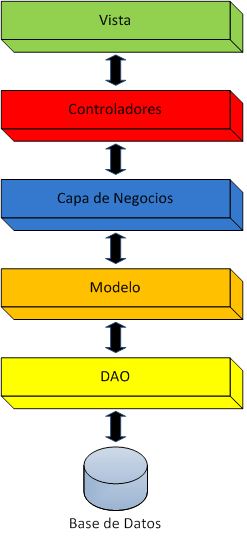
\includegraphics[scale=0.8]{images/ArquitecturaBM.png}
	\caption{Arquitectura del BM}
	\label{fig:ArquitecturaBM}
\end{figure}

\subsection{Base de Datos}
\noindent
La figura \ref{fig:dbBM} nos muestra el dise'no de la base de datos. 

\begin{figure}[h]
	\centering
		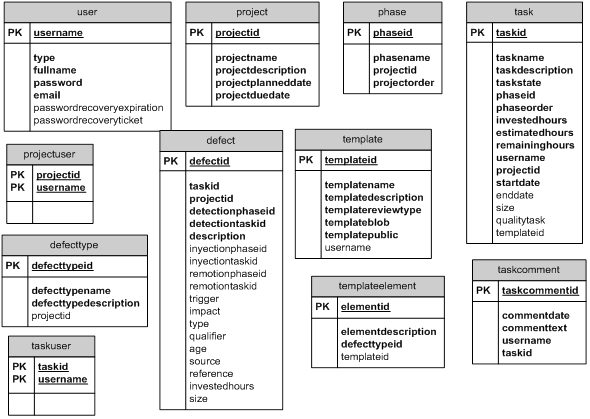
\includegraphics[scale=0.95]{images/dbBM.png}
	\caption{Base de Datos del BM}
	\label{fig:dbBM}
\end{figure}

Esta contiene las siguientes tablas:

\begin{itemize}
	\item \emph{User}. Contiene los usuarios del sistema.
	\item \emph{Project}. Contiene los proyectos del sistema.
	\item \emph{Phase}. Contiene las fases del sistema. Cada fase pertenece a un proyecto en espec'ifico.
	\item \emph{Task}. Contiene las tareas del sistema. Cada tarea est'a relacionada con un proyecto y con una fase del proyecto y puede ser una tarea de desarrollo o de calidad.
	\item \emph{Taskcomment}. Contiene los comentarios realizados en las tareas. Se relaciona con una tarea.
	\item \emph{Defect}. Contiene los defectos registrados en el sistema. Los defectos est'an relacionados con la tarea y la fase en la que fueron detectados.
	\item \emph{Template}. Contiene las plantillas que sirven como gu'ias para las actividades de calidad del sistema. Estas plantillas pueden ser p'ublicas o privadas. Inicia con la plantilla para lenguajes de prop'osito general propuesta por Humphrey\cite{Humphrey}.
	\item \emph{Templateelement}. Representa un elemento dentro de las plantillas de calidad, est'a relacionado a una plantilla en espec'ifico.
	\item \emph{Defecttype}. Contiene los tipos de defectos del sistema. Inicia con los tipos de defectos del PSP\cite{Humphrey}.
	\item \emph{Projectuser}. Es una tabla de soporte que ayuda a relacionar varios proyectos con varios usuarios.
	\item \emph{Taskuser}. Es una tabla de soporte que ayuda a relacionar varios usuarios con varias tareas.
\end{itemize}

\section{Funcionalidades del BM}
\label{sec:funcionalidadesdelbm}
\noindent
En esta secci'on se describir'an a detalle las secciones del BM. Encontraremos dos tipos de funcionalidades:

\begin{itemize}
	\item \emph{Funcionalidades de Administraci'on}. Estas funciones son aquellas necesarias para el correcto funcionamiento del sistema, como puede ser administraci'on de usuarios y de proyectos.
	\item \emph{Funcionalidades de Valor Agregado}. Estas funciones son aquellas que ayudan a las empresas a obtener los beneficios mencionados en la secci'on~\ref{sec:impacto}. En estas se har'a referencia a los objetivos que tienen y como son soportadas por la teor'ia.
\end{itemize}

\subsection{Administraci'on de Usuarios}
\noindent
Esta parte del sistema es meramente administrativa y solo los usuarios . Tiene las siguientes funcionalidades:

\begin{itemize}
	\item \emph{Alta de Usuarios}. Se registran nuevos usuarios especificando su nombre de usuario, nombre real, correo electr'onico, privilegios y contrase'na.
	\item \emph{Modificaci'on de Usuarios}. Se pueden editar los campos dados de alta en el Alta excepto la contrase'na.
	\item \emph{Cambio de Contrase'na}. Existe una pantalla especial para el cambio de contrase'na y recuperaci'on de esta en caso de haberla perdido.
	\item \emph{Eliminaci'on de Usuarios}. Se pueden eliminar los usuarios siempre y cuando no sea el usuario ``admin'' (usuario por default del sistema) y no est'e enrolado en ning'un proyecto.
\end{itemize}

\subsection{Administraci'on de Recursos}
\noindent
Otra parte del sistema administrativa pero con su grado de importancia. En esta secci�n un usuario con privilegios de administrador puede asignar a los diferentes usuarios del sistema a los proyectos existentes. Un usuario al ser asignado a un proyecto obtiene autom�ticamente la visibilidad de este.

\subsection{Administraci'on de Proyectos}
\noindent
Esta parte del sistema permite al administrador las siguientes funcionalidades:

\begin{itemize}
	\item \emph{Alta de Proyectos}. Se dan de alta nuevos proyectos especificando nombre del proyecto, descripci'on breve, fecha de entrega planeada y fecha de entrega real. Despu'es de dar de alta un proyecto se pasa a la creaci'on de su ciclo de vida.
	\item \emph{Modificaci'on de Proyectos}. Se pueden modificar los datos de los proyectos registrados en su alta. Aparte se especifica la fase actual en la que se encuentra el proyecto.
	\item \emph{Eliminaci'on de Proyectos}. Los proyectos pueden ser eliminados solamente cuando no tengan informaci'on registrada dentro de estos.
\end{itemize}

\subsection{Ciclo de Vida de Proyectos}
\label{sec:ciclodevidadeproyectos}
\noindent
El BM permite al administrador o al l'ider de proyecto la creaci'on de un ciclo de vida propio para el proyecto, o la selecci'on de uno predefinido que puede ser:

\begin{itemize}
	\item \emph{Cascada}. Es el ciclo de vida m'as cl'asico de los proyectos de desarrollo de software. Tiene las fases de Requerimientos, Dise'no, Codificaci'on, Pruebas y Mantenimiento.
	\item \emph{Iterativo}. Es el ciclo de vida preferido por los proyectos desarrollados en empresas con filosof'ias 'agiles. Este ciclo es una variaci'on del ciclo de vida de cascada, pero en vez de realizar el dise'no, la codificaci'on y las pruebas completas en una sola ocasi'on, dividen estas tres tareas en varias iteraciones para enfrentar los posibles cambios.
\end{itemize}

La figura \ref{fig:SSciclo1BM} nos muestra la pantalla donde se permite elegir los ciclos de vida. Una vez seleccionado un ciclo de vida default o comenzando a crear uno propio se pueden agregar, modificar o eliminar las fases existentes como se muestra en la figura \ref{fig:SSciclo2BM}. Una fase no puede ser eliminada una vez que tenga actividades registradas. Los datos que contiene una fase de un proyecto son: Nombre, tipo, descripci'on y orden en el proyecto.

Los tipos de fase predefinidos en el BM son los siguientes:

\begin{itemize}
	\item \emph{Requerimientos}. Esta es la fase donde se realiza la licitaci'on y el an'alisis de los requerimientos del proyecto.
	\item \emph{Dise'no}. En esta fase se toman las decisiones m'as importantes respecto a como ser'a construido el proyecto. Lo que se realice en esta fase determinar'a como es que el proyecto funcionar'a y si tendr'a 'exito o no. Los productos de trabajo de esta fase m'as comunes son la arquitectura y el dise'no detallado.
	\item \emph{Codificaci'on}. En esta fase se construye el sistema, tambi'en es llamada fase de construcci'on o programaci'on. Es la etapa de programaci'on y la primera que nos viene a la mente en el desarrollo de software.
	\item \emph{Revisi'on}. Esta fase puede ser utilizada como comod'in. Se incluy'o en caso de que el equipo de desarrollo decida agregar alguna fase completa de revisi'on de los productos de otra fase. Ya que el costo de los errores aumenta exponencialmente conforme avanza de fases el proyecto\cite{Lazic2009}, entonces es muy importante evitar la inyecci'on de errores en fases tempranas como Requerimientos y Dise'no, as'i que podr'ia incluirse una fase completa para realizar actividades como inspecciones al dise'no y a los requerimientos. En caso de que se decida no utilizar una fase completa para revisiones, es muy importante que al menos se realicen revisiones personales al trabajo realizado.
	\item \emph{Pruebas}. Esta etapa corresponde a las pruebas cl'asicas. Se recomienda al menos la realizaci'on de pruebas unitarias y de sistema.
	\item \emph{Mantenimiento}. Esta fase es cuando el sistema ha salido a producci'on y se contin'uan agregando nuevas funcionalidades o defectos encontrados por el cliente. El objetivo del BM es que no haya ning'un defecto reportando por el cliente.
\end{itemize}

\begin{figure}[h]
	\centering
		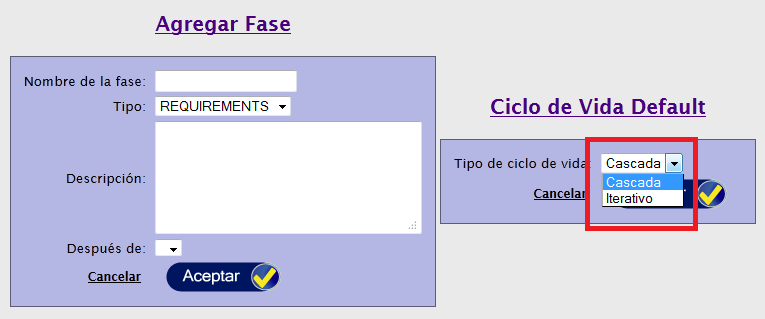
\includegraphics[scale=0.8]{images/SSciclo1BM.png}
	\caption{Ciclo de Vida Default}
	\label{fig:SSciclo1BM}
\end{figure}

\begin{figure}[h]
	\centering
		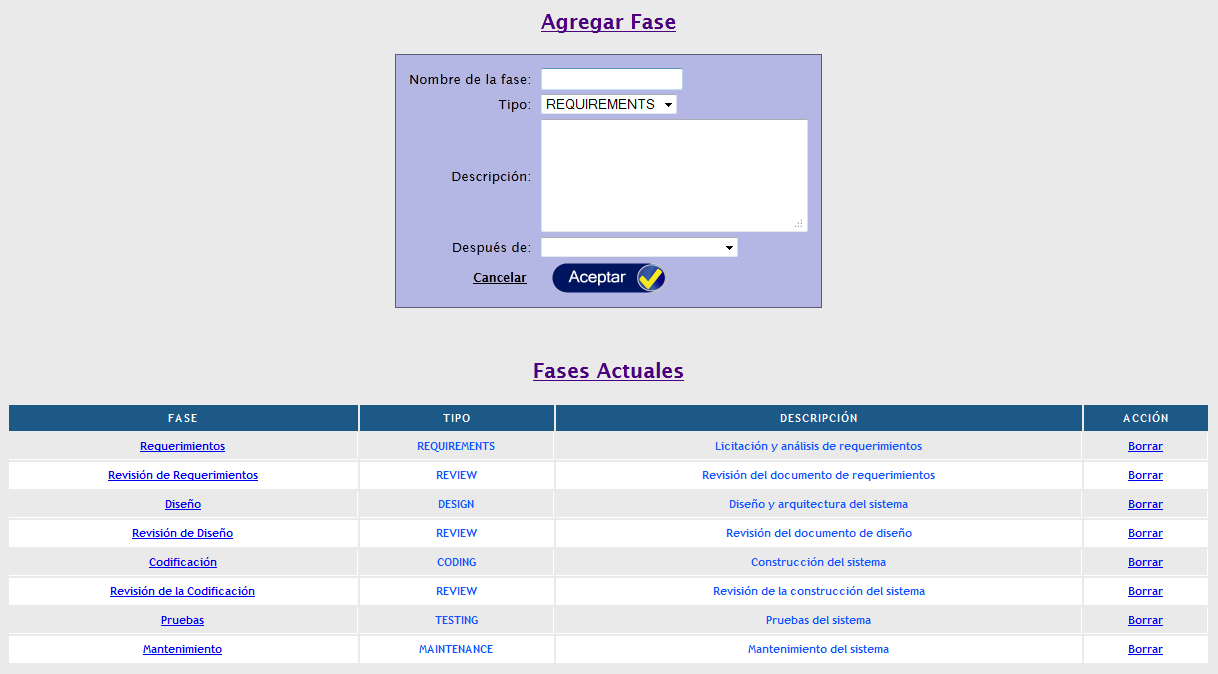
\includegraphics[scale=0.5]{images/SSciclo2BM.png}
	\caption{Edici'on del Ciclo de Vida}
	\label{fig:SSciclo2BM}
\end{figure}

Es importante destacar que la definici'on del ciclo de vida es el primer paso para iniciar la planeaci'on del proyecto. La planeaci'on es una de las pr'acticas recomendadas por \cite{Humphrey2002} para realizar la administraci'on racional. Si una organizaci'on quiere tener 'exito en el negocio del software es clave la planeaci'on del proyecto.

Para el uso correcto del BM y obtener su mayor potencial se recomienda una definici'on a conciencia del ciclo de vida. Una vez definido el ciclo de vida se puede pasar a la definici'on de las tareas dentro de cada fase. Tambi'en es de suma importancia que cada una de estas tareas cuente con su actividad de revisi'on, para fomentar la cultura de la prevenci'on antes de las pruebas.

\subsection{Administraci'on  y Seguimiento de Actividades}
\label{sec:administracionyseguimientodeactividades}
\noindent
El registro, actualizaci'on y medici'on de las actividades realizadas dentro de un proyecto es clave para hacer un trabajo de calidad. Lo que es medido es administrado, y lo que es administrado se hace correctamente, en cambio, lo que no es medido no se administra y por lo tanto no se termina\cite{Humphrey2002}. 

El BM facilita la labor de la planeaci'on y administraci'on de actividades por medio de distintas funcionalidades:

\begin{itemize}
	\item La creaci'on de un ciclo de vida para el proyecto como se explic'o en la secci'on \ref{sec:ciclodevidadeproyectos}.
	\item El alta, baja y modificaci'on de actividades.
	\item El seguimiento y actualizaci'on de las actividades.
\end{itemize}

El BM tiene dos tipos de actividades:

\begin{itemize}
	\item \emph{Actividades de Desarrollo}. En esta categor'ia caen todas las actividades relacionadas con el proceso de desarrollo de software en las cuales se generan productos de trabajo. Ejemplos de estas son: Licitaci'on de requerimientos, dise'no detallado del m'odulo de un sistema, programaci'on, pruebas unitarias entre otras. Este tipo de actividades tienen subtipos, estos son los siguientes:	
	\begin{itemize}
		\item \emph{REQUIREMENTS}. Actividades relacionadas a una fase de requerimientos.
		\item \emph{DESIGN}. Actividades relacionadas a una fase de dise'no.
		\item \emph{DEVELOPMENT}. Actividades relacionadas a la fase de construcci'on.
		\item \emph{TESTING}. Actividades relacionadas con alguno de los tipos de prueba mencionados en la secci'on \ref{sec:pruebasdesoftware}.
	\end{itemize}
\end{itemize}

\begin{itemize}
	\item \emph{Actividades de Calidad}. Son las actividades de prevenci'on y evaluaci'on realizadas en el proyecto de desarrollo las cuales nos ayudan a evitar la inyecci'on de defectos o a detectarlos lo antes posible dentro del ciclo de desarrollo. Las actividades de calidad que maneja el BM, las cuales fueron descritas a detalle en la secci'on \ref{sec:tecnicasdedetecciondedefectos}, son las siguientes:
	\begin{itemize}
		\item \emph{PERSONAL REVIEW}. Actividades donde se realiza una revisi'on personal a un producto de trabajo.
		\item \emph{PEER REVIEW}. Actividades donde se realiza una revisi'on entre colegas de un producto de trabajo.
		\item \emph{WALKTHROUGH}. Actividades donde se realiza una caminata a un producto de trabajo.
		\item \emph{INSPECTION}. Actividades donde se realiza una inspecci'on a un producto de trabajo.
	\end{itemize}
\end{itemize}

Para obtener mayores beneficios del BM y tener un nivel 'optimo de calidad se recomienda la siguiente forma de trabajo:

\begin{itemize}
	\item Realizar al menos una revisi'on personal a cada producto de trabajo utilizando una plantilla de calidad. Por ejemplo cada que el desarrollador termine de programar un clase del sistema, realizar una revisi'on personal de esta apoy'andose con la plantilla de calidad default o una elaborada personalmente.
	\item Realizar una inspecci'on a cada producto mayor de trabajo. Un producto mayor de trabajo es un producto que representa el cierre de una fase, por ejemplo: El documento de requerimientos al terminar la fase de requerimientos, la arquitectura del sistema al terminar el dise'no conceptual, entre otros.	
\end{itemize}

Las funcionalidades b'asicas con las actividades tanto de desarrollo como de calidad son las siguientes:

\begin{itemize}
	\item \emph{Alta de actividades}. Se registra una nueva actividad en el sistema con los siguientes datos: Nombre de la tarea, tipo, fase, descripci'on, esfuerzo planeado, reponsable, fecha de inicio y fecha meta. La forma se puede ver en la figura \ref{fig:SSagregartareaBM}.
	\item \emph{Modificaci'on de actividades}. Se modifican los datos con los cuales se dieron de alta las actividades.
	\item \emph{Baja de actividades}. Una actividad puede ser dada de baja solo en el caso de que no tenga registrado esfuerzo.
\end{itemize}

\begin{figure}[h]
	\centering
		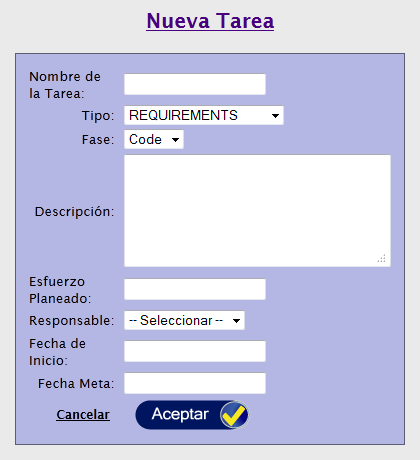
\includegraphics[scale=0.9]{images/SSagregartareaBM.png}
	\caption{Creaci'on de Actividades}
	\label{fig:SSagregartareaBM}
\end{figure}

El seguimiento de las actividades se muestra en la figura \ref{fig:SSseguirtarea1BM}. Esto nos permitir'a hacer un seguimiento y administraci'on adecuado de cada tarea. Se recomienda que diariamente el responsable de la actividad haga una actualizaci'on de esta con las siguientes consideraciones:

\begin{itemize}
	\item Escribir en el campo de Agregar Esfuerzo el n'umero de horas reales que le dedic'o a la tarea. Por ejemplo: Un desarrollador tiene como tarea programar la interfaz de un sistema un d'ia de trabajo; pero en el d'ia de 8 horas, pas'o 2 horas en juntas, otra hora revisando el correo electr'onico y una hora m'as en descansos, entonces ese d'ia debe reportar 4 horas al esfuerzo y no las 8 horas del d'ia. Esto es muy importante para que las empresas identifiquen las horas reales de trabajo que tienen los desarrolladores y as'i puedan hacer m'as eficiente el tiempo en la oficina.
	\item Si el esfuerzo restante se deja en 0 la actividad ser'a marcada como terminada, as'i que es importante que se estime el esfuerzo restante y se coloque en el campo respectivo. Esto ayudar'a a los desarrolladores a mejorar sus habilidades de estimaci'on y generar datos hist'oricos.
	\item Colocar el tama'no de la tarea en las unidades que maneje la empresa. Para el uso del BM se recomienda utilizar LOC para los programas por su facilidad al momento de calcular y lo com'un que es dentro de la industria, sin embargo se pueden utilizar otras m'etricas como puntos de funci'on. Esto tambi'en ayudar'a a crear datos hist'oricos y facilitar'a el dimensionamiento de futuros proyectos.
	\item Agregar comentarios para cada suceso importante que surja en las actividades. Los comentarios quedar'an registrados y ser consultados despu'es.
	\item Tener en cuenta que la Fecha Fin no es la fecha en que se finaliz'o la tarea, si no la fecha en que estaba planeado en que se finalizara. La fecha cuando se finaliza la tarea se registra de forma autom'atica cuando el estatus de la tarea pasa a COMPLETADA. 
\end{itemize}

\begin{figure}[h]
	\centering
		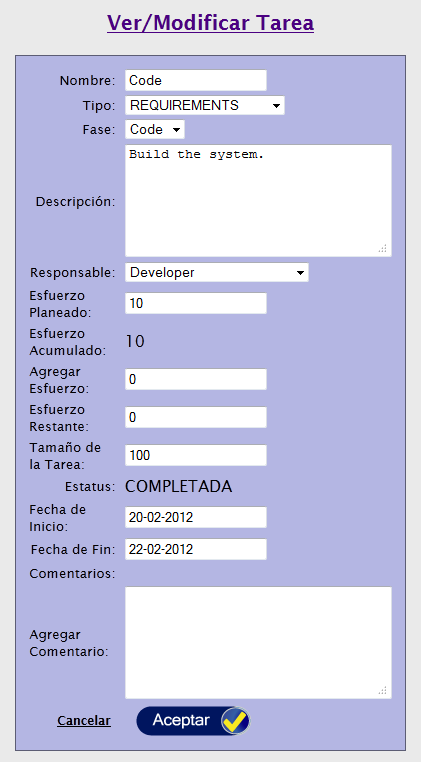
\includegraphics[scale=0.7]{images/SSseguirtarea1BM.png}
	\caption{Seguimiento de Actividades}
	\label{fig:SSseguirtarea1BM}
\end{figure}

Las actividades de calidad se administran de manera similar a las actividades de desarrollo. Las diferencias principales son su enfoque y el uso de plantillas de calidad. Mientras que las actividades de desarrollo tienen como principal objetivo construir el sistema mediante la creaci'on de productos de trabajo, las actividades de calidad tienen como objetivo revisar estos productos de trabajo, para liberarlos de defectos y evitar que estos avancen durante el ciclo de vida.

Es de suma importancia evitar que los defectos avancen en el ciclo de vida de desarrollo del sistema, ya que como se explic'o en la secci'on \ref{sec:elcostorealdelosdefectosdesoftware}, el esfuerzo, y por lo tanto el costo, de remover estos defectos aumenta exponencialmente conforme el defecto cambia de fase.

Entonces las actividades de calidad son realizadas ya sea inmediatamente despu'es de terminar un producto de trabajo o al final de la fase. Estas actividades deben de ser apoyadas con una plantilla de calidad, la cual servir'a de gu'ia en la realizaci'on de la actividad. Estas plantillas fueron descritas a mayor profundidad en la secci'on \ref{sec:listadechequeoderevisiondecodigo} y su uso dentro del BM ser'a descrito en la secci'on \ref{sec:administraciondeplantillasdecalidad}.

\subsection{Administraci'on  y Seguimiento de Defectos}
\label{sec:administracionyseguimientodedefectos}
\noindent
El BM toma su nombre de la funcionalidad explicada en esta secci'on. El registro, seguimiento y administraci'on correcta de los defectos introducidos en el desarrollo de software es fundamental para asegurar su calidad. Tan solo el registro de los defectos que son inyectados provoca una disminuci'on del 30\% en la densidad de defectos de un proyecto de software\cite{Humphrey}. La correcta administraci'on de defectos permite generar estad'isticas y m'etricas para conocer los defectos que:

\begin{itemize}
	\item Se encuentran en el programa final o en el periodo de pruebas;
	\item Aquellos que ocurren m'as frecuentemente;
	\item Aquellos que son m'as dif'iciles o costosos de corregir;
	\item Aquellos en los que se pueden realizar acciones preventivas sencillas;
	\item Aquellos que m'as nos molestan.
\end{itemize}

Las funcionalidades b'asicas para la administraci'on de defectos son las siguientes:

\begin{itemize}
	\item \emph{Alta de defectos}. Es el registro de un nuevo defecto. La informaci'on requerida para dar de alta es la siguiente: El nombre del defecto, una descripci'on breve del defecto, la fase actual en que se encuentra el proyecto (se coloca autom'aticamente) y la tarea donde fue detectado el defecto. Ver la figura \ref{fig:SSdefectos1BM}.
	\item \emph{Baja de defectos}. El defecto puede ser borrado siempre y cuando tenga ENVIADO de estatus y sin esfuerzo agregado.
	\item \emph{Modificaci'on de defectos}. Es el seguimiento de defectos propiamente, ser'a explicado a m'as detalle a continuaci'on.
\end{itemize}

\begin{figure}[h]
	\centering
		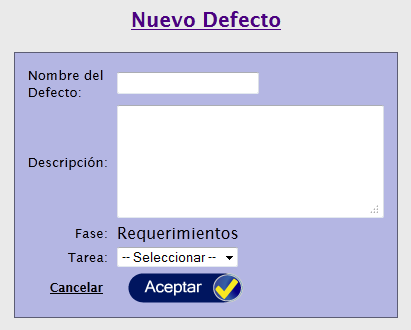
\includegraphics[scale=0.9]{images/SSdefectos1BM.png}
	\caption{Agregar Nuevo Defecto}
	\label{fig:SSdefectos1BM}
\end{figure}

La modificaci'on de defectos se refiere al seguimiento que se le dar'a al defecto desde que es reportado hasta que es corregido o cancelado. Para el seguimiento existen varios campos editables los cuales contienen la informaci'on de la clasificaci'on ortogonal de defectos\cite{Chillarege1992}, la cual fue explicada a detalle en la secci'on \ref{sec:clasificacionortogonaldedefectos}, y otros propuestos para el BM. A continuaci'on se explica cada uno de estos campos (ver figura \ref{fig:SSdefectos2BM}):

\begin{itemize}
	\item \emph{Nombre}. Es un nombre que se le asigna al defecto para identificarlo r'apidamente.
	\item \emph{Descripci'on}. Esta debe de decir a grandes rasgos los s'intomas del defecto para poder replicarlo.
	\item \emph{Responsable}. Es la persona del equipo de trabajo encargada de corregir el defecto, no necesariamente es quien inyect'o el defecto.
	\item \emph{Fecha de Apertura}. Se asigna autom'aticamente cuando se da de alta el defecto.
	\item \emph{Fecha de Cierre}. Se asigna autom'aticamente cuando el estatus del defecto pasa a CORREGIDO o CANCELADO.
	\item \emph{Fase de Detecci'on}. Se asigna autom'aticamente dependiendo de la fase actual en que se encuentre el proyecto.
	\item \emph{Tarea de Detecci'on}. Es la tarea que se estaba realizando cuando se detect'o el defecto. Es importante destacar que los defectos pueden ser encontrados ya sea en tareas de desarrollo o de calidad. Por ejemplo: Un programador puede encontrar un defecto en el dise'no al momento de implementarlo.
	\item \emph{Fase de Inyecci'on}. Este campo no es obligatorio. Representa la fase en que el defecto fue inyectado.
	\item \emph{Tarea de Inyecci'on}. Este campo no es obligatorio. Representa la tarea en que el defecto fue inyectado.
	\item \emph{Fase de Remoci'on}. Este campo es obligatorio para cambiar el estatus del defecto a CORREGIDO. Representa la fase donde el defecto fue corregido.
	\item \emph{Tarea de Remoci'on}. Este campo es obligatorio para cambiar el estatus del defecto a CORREGIDO. Representa la tarea donde el defecto fue corregido.
	\item \emph{Esfuerzo Acumulado}. Al igual que en las actividades, representa el esfuerzo realizado hasta el momento en la remoci'on del defecto.
	\item \emph{Agregar Esfuerzo}. Funciona igual que en las actividades. Se agrega el esfuerzo invertido en el defecto hasta el momento, si se deja en cero entonces el estatus del defecto pasa a CORREGIDO.
	\item \emph{Estatus}. El defecto puede tener cuatro estados:
	\begin{itemize}
		\item \emph{ENVIADO}. Es el estatus inicial del defecto el cual tiene una vez que este es registrado.
		\item \emph{ACEPTADO}. Es el estatus que el responsable del defecto coloca cuando este determina que lo reportado si es un defecto y se dispone a corregirlo.
		\item \emph{CANCELADO}. Es el estatus del defecto cuando se decide que el defecto no ser'a corregido o no es realmente un defecto.
		\item \emph{CORREGIDO}. Es el estatus que se coloca cuando el responsable ha corregido el defecto.
	\end{itemize}
	\item \emph{Tipo de Defecto}. Los tipos de defectos ser'an explicados a detalle en la secci'on \ref{sec:administraciondetiposdedefectos}.
	\item \emph{Edad}. Es un campo de la clasificaci'on ortogonal de defectos\cite{Chillarege1992}. Fue explicado a detalle en la secci'on \ref{sec:clasificacionortogonaldedefectos}.
	\item \emph{Fuente}. Es un campo de la clasificaci'on ortogonal de defectos\cite{Chillarege1992}. Fue explicado a detalle en la secci'on \ref{sec:clasificacionortogonaldedefectos}.
	\item \emph{Referencia}. Este campo representa si el defecto fue inyectado cuando se correg'ia otro defecto. Contiene el identificador 'unico de otro defecto.
	\item \emph{Agregar Comentario}. Al igual que para las actividades, se pueden agregar comentarios para mencionar cualquier situaci'on relevante al defecto.
\end{itemize}

\begin{figure}[h]
	\centering
		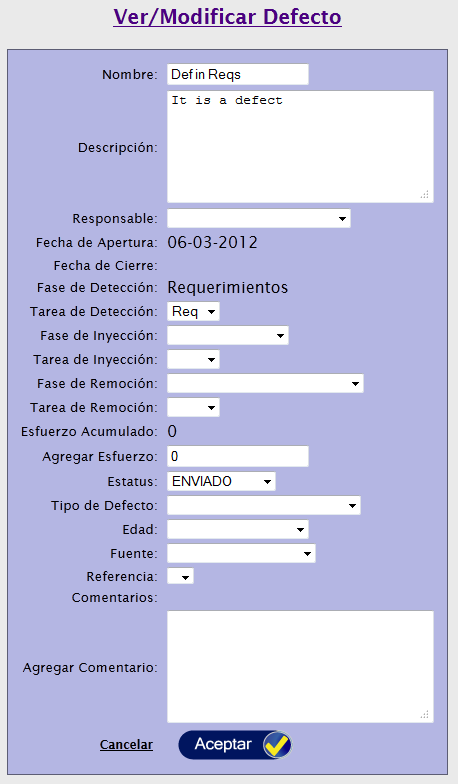
\includegraphics[scale=0.7]{images/SSdefectos2BM.png}
	\caption{Seguimiento de Defectos}
	\label{fig:SSdefectos2BM}
\end{figure}

Para que las empresas obtengan los beneficios del BM se recomiendan las siguientes actividades como m'inimo en la administraci'on y seguimiento de defectos:

\begin{itemize}
	\item Registrar el momento en el que los defectos sean detectados, si no se hace entonces se olvida y el defecto nunca ser'a registrado.
	\item Agregar el esfuerzo real que tom'o el defecto. Al igual que en las actividades registrar solo el tiempo efectivo que se tom'o para corregir el defecto.
	\item Clasificar correctamente el defecto seg'un su tipo.
	\item Agregar nuevos tipos de defectos si es que lo requiere la organizaci'on de software. Ver secci'on \ref{sec:administraciondetiposdedefectos}.
	\item Encontrar las fases y tareas de inyecci'on y remoci'on de cada defecto.
	\item Al realizar la correcci'on del defecto utilizar las plantillas de calidad que se utilizan para una actividad de desarrollo. Esto con la finalidad de asegurarnos de no inyectar nuevos defectos al corregir un defecto previo.
\end{itemize}

Estas acciones permitir'an al BM identificar cuales son los tipos m'as comunes de defectos, que defectos son m'as costosos de corregir, en que fases se inyectan m'as defectos y otras m'etricas valiosas para que las organizaciones puedan establecer estrategias para mejorar la calidad.

\subsection{Administraci'on de Tipos de Defectos}
\label{sec:administraciondetiposdedefectos}
\noindent
Los defectos pueden ser clasificados por su tipo. Por ejemplo, no es lo mismo un error de sintaxis que un error en el dise'no, o un error en la l'ogica de un algoritmo. Es por esto que el BM permite la administraci'on de los tipos de defectos, es decir, permite el alta, baja y modificaci'on de estos tipos. El BM sugiere al menos utilizar los defectos que propone Humphrey en el PSP \cite{Humphrey} (ver tabla \ref{DefectosPSP2}). Sin embargo este tipo de defectos son muy gen'ericos, y pueden no ser suficientes para todas las organizaciones de software, as'i que se recomienda agregar tipos de defectos seg'un las necesidades de cada organizaci'on.

\begin{table}[htbp]
	\centering
		\begin{tabular}{| l | l | l |}
			\hline
			\textbf{N'umero de Tipo} & \textbf{Nombre del Tipo} & \textbf{Descripci'on} \\ \hline
			10 & Documentaci'on & Comentarios y mensajes. \\ \hline
			20 & Sintaxis & Ortograf'ia, puntuaci'on y tipos. \\ \hline
			30 & Paquete & Administraci'on, librer'ias y versiones. \\ \hline
			40 & Asignaci'on & Declaraci'on, nombres duplicados y l'imites. \\ \hline
			50 & Interface & Procedimientos, referencias, I/O y formatos. \\ \hline
			60 & Chequeo & Mensajes de error y chequeos inadecuados. \\ \hline
			70 & Datos & Estructura y contenido. \\ \hline
			80 & Funci'on & L'ogica, apuntadores, ciclos, etc. \\ \hline
			90 & Sistema & Configuraci'on, tiempo y memoria. \\ \hline
			100 & Medio Ambiente & Dise'no, compilaci'on y pruebas.\\
			\hline
		\end{tabular}
	\caption{Clasificiaci'on de Defectos del PSP}
	\label{DefectosPSP2}
\end{table}

\subsection{Administraci'on de Plantillas de Calidad}
\label{sec:administraciondeplantillasdecalidad}
\noindent
El BM es un sistema que sirve como gu'ia para la implementaci'on de estrategias de calidad en las organizaciones peque'nas y medianas de software. Una herramienta muy importante que brinda el BM a estas organizaciones son las plantillas de calidad. Estas plantillas de calidad son el equivalente a las listas de chequeo mencionadas por Humphrey en el PSP\cite{Humphrey} y revisadas a detalla en la secci'on \ref{sec:listadechequeoderevisiondecodigo} del presente Trabajo de Tesis.

Las plantillas de calidad son entonces gu'ias especializadas para guiar las actividades de detecci'on de defectos. El BM tiene la capacidad de dar de alta (ver figura \ref{fig:SSplantillas2BM}), modificar y eliminar plantillas de calidad. Las plantillas de calidad pueden ser p'ublicas o privadas, es decir, si el administrador o el l'ider de proyecto pueden crear una plantilla para que sea visible por todos los desarrolladores de la organizaci'on, o cualquier usuario puede crear una plantilla para solo ser utilizada por 'el.

\begin{figure}[h]
	\centering
		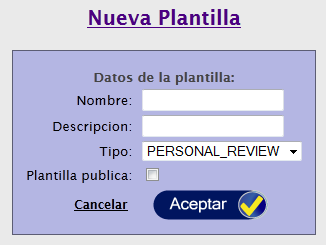
\includegraphics[scale=0.9]{images/SSplantillas2BM.png}
	\caption{Crear Nueva Plantilla de Calidad}
	\label{fig:SSplantillas2BM}
\end{figure}

Dentro del BM tienen las siguientes partes (ver figura \ref{fig:SSplantillas1BM}):

\begin{itemize}
	\item Una serie de categor'ias las cuales se obtienen a partir de los tipos de defectos.
	\item Una serie de tareas o estrategias dentro de cada categor'ia para poder detectar los tipos de defectos.
\end{itemize}

\begin{figure}[h]
	\centering
		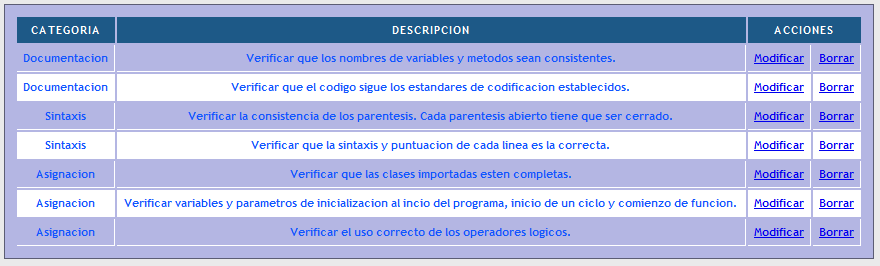
\includegraphics[scale=0.7]{images/SSplantillas1BM.png}
	\caption{Editar Plantilla de Calidad}
	\label{fig:SSplantillas1BM}
\end{figure}

La figura \ref{fig:SSplantillas1BM} nos muestra una plantilla de calidad para realizar revisiones personales a c'odigos escritos en lenguajes de prop'osito general como Java, C++, Pascal, etc. Como se puede observar, existen tres columnas:

\begin{itemize}
	\item \emph{Categor'ia}. Esta columna nos muestra el tipo de defecto.
	\item \emph{Descripci'on}. Es la descripci'on de la actividad o estrategia a seguir.
	\item \emph{Acciones}. Son acciones simples para modificar o borrar la estrategia escrita.
\end{itemize}

La plantilla propuesta dentro del BM tiene las siguientes estrategias para detectar defectos, se mencionar'a el tipo de defecto que busca detectar, la estrategia y una breve explicaci'on (ver Tabla \ref{plantilladecalidadbm}).

\begin{table}[htbp]
	\centering
		\begin{tabular}{| p{3.5cm} | p{5cm} | p{6.5cm} |}
			\hline
			\textbf{Tipo de Defecto} & \textbf{Estrategia} & \textbf{Explicaci'on} \\ \hline
			Documentaci'on & Verificar que los nombres de variables y m'etodos sean consistentes. & Busca que los nombres de los m'etodos y las variables tengan relaci'on con su uso dentro del c'odigo. Con esto se asegura de que el c'odigo sea le'ible y m'as f'acil de ser entendido por un tercero o en un futuro. \\ \hline
			Documentaci'on & Verificar que el c'odigo sigue los est'andares de codificaci'on establecidos. & Busca asegurarse que el c'odigo escrito siga los est'andares de codificaci'on de la organizaci'on de software para que el c'odigo elaborado por todos los desarrolladores tenga un mismo formato. \\ \hline
			Sintaxis & Verificar la consistencia de los par'entesis. Cada par'entesis abierto tiene que ser cerrado. & Asegura que el c'odigo no tenga problemas relacionados a las parejas de par'entesis y llaves a trav'es del c'odigo. \\ \hline
			Sintaxis & Verificar que la sintaxis y puntuaci'on de cada l'inea es la correcta. & Asegura que el c'odigo al momento de compilar tenga el menor n'umero de errores de sintaxis posible y evitar tomar mucho tiempo en compilaci'on. \\ \hline
			Sintaxis & Verificar que las clases importadas est'en completas. & Evita que al momento de la compilaci'on se tengan errores debido a que una funci'on no es encontrada a causa de no existir la librer'ia. \\ \hline
			Asignaci'on & Verificar variables y par'ametros de inicializaci'on al inicio del programa, ciclo y funci'on. & Asegura que una variable no tenga un valor nulo al momento de ejecuci'on. \\ \hline
			Asignaci'on & Verificar el uso correcto de los operadores l'ogicos. & Asegura que no haya problemas con los operadores l'ogicos al momento de realizar condiciones. \\ 
			\hline
		\end{tabular}
	\caption{Plantilla de Calidad BM}
	\label{plantilladecalidadbm}
\end{table}

\subsection{Reportes}
\label{sec:reportes}
\noindent
Los reportes del BM nos permiten analizar el desempe'no de los distintos aspectos de la organizaci'on de software. Nos permite conocer estad'isticas por desarrollador, por proyecto y por organizaci'on. Los l�deres de proyecto tienen acceso a los reportes para desarrolladores y sus proyectos, mientras que los administradores tienen acceso a todos los reportes. Estos reportes son generados a partir de toda la informaci'on ingresada por los usuarios del BM en las actividades y los defectos. As'i que para que los reportes sean 'utiles y con informaci'on fidedigna deben seguirse a conciencia las recomendaciones de las secciones \ref{sec:administracionyseguimientodeactividades} y \ref{sec:administracionyseguimientodedefectos}. 

Otro aspecto importante a remarcar, es que el BM es flexible en cuanto las unidades de tama'no utilizadas para medir los productos de trabajo del desarrollo de software. Se recomienda el uso de LOC para los programas y hojas de documentaci'on para los dem'as productos, sin embargo cada organizaci'on puede reportar lo que le sea m'as conveniente. Sin embargo es de suma importancia no mezclar unidades, si se comenz'o a registrar el tama'no de los programas en LOC y despu'es se hace en puntos de funci'on, es un hecho que la informaci'on presentada en los reportes ser'a inconsistente. Entonces, cada organizaci'on debe de mantener las mismas unidades, o iniciar con una nueva instalaci'on del BM si se desea cambiarlas.

A partir de analizar los reportes tanto las organizaciones de software, como los l'ideres de proyecto y los desarrolladores podr'an plantear estrategias para mejorar en las 'areas de oportunidad y as'i mejorar su productividad y calidad en el desarrollo de software. El BM nos da reportes en cuatro 'areas distintas: Generales, costo de la calidad, t'ecnicas de detecci'on de defectos y caracterizaci'on de defectos. La tabla\ref{ReportesBM} nos muestra los reportes que existen, organizados por 'area y mostrando al nivel de la organizaci'on que se pueden aplicar:

\begin{table}[htbp]
	\centering
		\begin{tabular}{|p{5cm}|p{5cm}|p{5cm}|} \hline
		\textbf{Categor'ia} & \textbf{Reportes} & \textbf{Nivel(es)}\\ \hline
		\multirow{4}{*}{Generales} 
		& Tiempo por Fase & Proyecto \\
		& Productividad por Fase & Proyecto \\
		& Yield por Fase & Proyecto \\
		& Resumen General & Proyecto \\ \hline
		\multirow{4}{*}{CoQ} 
		& Productividad Compuesta & Usuario, Proyecto, Organizaci'on \\
		& ROI de Proyecto/Empresa & Proyecto, Organizaci'on \\
		& ROI de T'ecnicas de Detecci'on & Proyecto, Organizaci'on \\
		& CoQ vs CNQ & Proyecto, Organizaci'on \\ \hline
		\multirow{5}{*}{T'ecnicas de Detecci'on} 
		& Yield por T'ecnica de Detecci'on & Proyecto, Organizaci'on \\
		& Esfuerzo por T'ecnica de Detecci'on & Proyecto, Organizaci'on \\
		& Eficiencia por T'ecnica de Detecci'on & Proyecto, Organizaci'on \\
		& Raz'on de Revisi'on por T'ecnica de Detecci'on & Proyecto, Organizaci'on \\
		& N'umero de Defectos por T'ecnica de Detecci'on & Proyecto, Organizaci'on \\ \hline
		\multirow{3}{*}{Defectos} 
		& Densidad de Defectos & Usuario, Proyecto, Organizaci'on \\
		& N'umero de Defectos por Tipo & Usuario, Proyecto, Organizaci'on\\
		& Defectos Inyectados y Removidos por Fase & Usuario, Proyecto, Organizaci'on \\ \hline
		\end{tabular}
	\caption{Reportes BM}
	\label{ReportesBM}
\end{table}

Para el presente Trabajo de Tesis se har'a un enfoque especial a los reportes relacionados con el CoQ. A continuaci'on se detallar'an los reportes pertinentes y se explicar'a la clase de informaci'on que le brindan a las organizaciones.

\subsubsection{Tiempo por Fase}
\label{sec:tiempoporfase}
\noindent
Este es el primer reporte general que ofrece el BM. Este reporte solo se presenta a nivel proyecto y es bastante simple. Solo nos dice el esfuerzo invertido en cada fase en el proyecto elegido. Aunque puede sonar algo trivial el reporte nos puede demostrar el tiempo que gastan las organizaciones de software en pruebas, que es en promedio la mitad del tiempo total del proyecto \cite{Humphrey}. Por medio del an'alisis de este reporte se pueden tomar estrategias como invertir una mayor cantidad de tiempo en la fase de dise'no y en las actividades de calidad para reducir el tiempo que toma la fase de pruebas.

\subsubsection{Productividad por Fase}
\label{sec:ProductividadporFase}
\noindent
Productividad por fase es un reporte a nivel proyecto. Este reporte nos dice la productividad que hubo en cada fase. Es importante mencionar que la productividad en cada fase est'a en unidades distintas. Por ejemplo: Lo m'as com'un ser'ia encontrar la fase de programaci'on medida en LOC o puntos de funci'on por hora, mientras que fases como dise'no o requerimientos estar'ian medidas en hojas de documentaci'on por hora. La productividad se calcula con la siguiente f'ormula:

\begin{math}P = \frac{S}{E}\end{math}

Donde:

\begin{itemize}
	\item P: Productividad.
	\item S: Tama'no del producto.
	\item E: Esfuerzo de la fase.
\end{itemize}

Organizaciones maduras en el desarrollo de software tienen una productividad promedio de 20 l'ineas de c'odigo por hora e inyectan un error cada diez LOC \cite{Humphrey2002}. A partir de estos valores podemos comenzar a comparar nuestra organizaci'on con la industria.

\subsubsection{Yield por Fase}
\label{sec:YieldporFase}
\noindent
El Yield mida la eficiencia de cada fase en la detecci'on de defectos. El Yield de una fase es el porcentaje de defectos de producto totales que son removidos en una fase. Por ejemplo: Al final del proyecto se sabe que se inyectaron 100 defectos al final de la fase de codificaci'on, sin embargo 50 de estos defectos fueron removidos en esta misma fase, por lo tanto el Yield de la fase de codificaci'on para dicho proyecto es del 50\%.

Con este reporte las organizaciones de software pueden medir la efectividad removiendo defectos que tienen en cada fase. Un Yield de fase adecuado es del 70\% [CITA]. La f'ormula para calcular el Yield es la siguiente:

\begin{math}Y = \frac{DD}{DT}\end{math}

Donde:

\begin{itemize}
	\item Y: Yield.
	\item DD: Defectos Detectados en la Fase.
	\item DT: Defectos Totales del Proyecto.
\end{itemize}

\subsubsection{Resumen General}
\label{sec:ResumenGeneral}
\noindent
El resumen general es un reporte a nivel proyecto. Es una herramienta muy poderosa con la que cuenta el BM para analizar la calidad con la que se est'a construyendo el desarrollo de software. Muestra una radiograf'ia actual con las m'etricas m'as importantes de calidad de software (ver secci'on \ref{sec:metricasdecalidad}). Un ejemplo de este reporte lo podemos ver en la figura \ref{fig:SSreportes1BM}.

\begin{figure}[h]
	\centering
		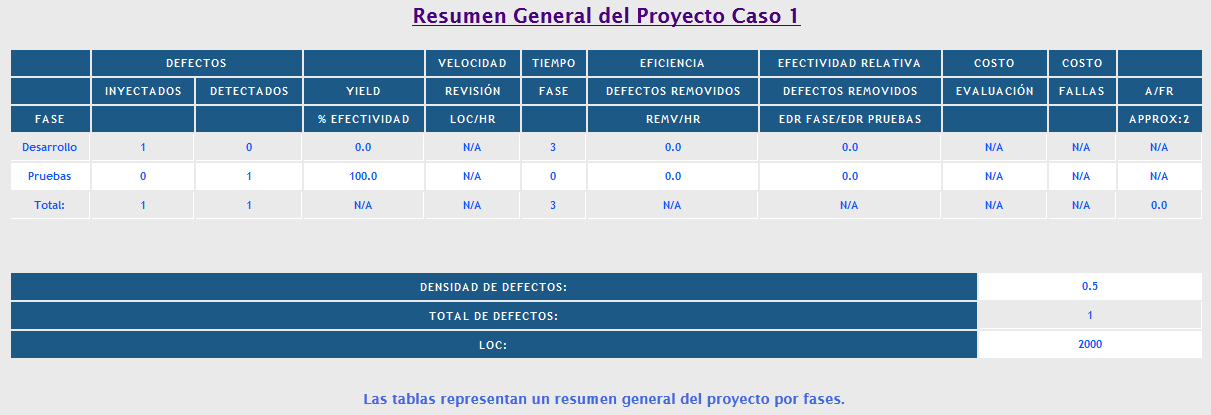
\includegraphics[scale=0.6]{images/SSreportes1BM.png}
	\caption{Resumen General}
	\label{fig:SSreportes1BM}
\end{figure}

A continuaci'on se describir'an a detalle las partes del reporte:

\begin{itemize}
	\item La primera columna con nombre FASE, representa las fases que tiene el proyecto en cuesti'on.
	\item La segunda y tercer columna representan los defectos. La segunda muestra los defectos que se inyectaron en la fase determinada y la tercera muestra los defectos que fueron detectados en esa fase.
	\item La cuarta columna muestra el Yield (la eficiencia de detecci'on de defectos) de cada fase. Se recomienda un Yield m'inimo de 70\% para cada fase\cite{Humphrey}. Si no se tiene el Yield adecuado se pueden tomar estrategias como integrar nuevas actividades de calidad a la fase, o mejorar la forma en que se hacen las actividades de calidad actuales.
	\item La quinta columna presenta la Raz'on de Revisi'on de las actividades de calidad de cada fase. En otras palabras es la velocidad con que se realizan las revisiones. M'as detalles acerca de la Tasa de Revisi'on en la secci'on \ref{sec:RazonporTecnicadeDeteccion}.
	\item La sexta columna simplemente muestra el tiempo total que ha tomado cada fase. En organizaciones con una pobre calidad en el desarrollo de software la fase de pruebas toma hasta el 50\% del tiempo total del proyecto[CITA]. El objetivo del BM es ayudar a las organizaciones de desarrollo de software a llegar a la fase de pruebas con cero defectos.
	\item La s'eptima columna representa la eficiencia removiendo defectos de cada fase. Se mide en defectos removidos por hora.
	\item La octava columna presenta la efectividad relativa detectando defectos. Esta m'etrica hace una comparaci'on entre la eficiencia detectando defectos de una fase cualquiera contra la eficiencia de la fase de pruebas. Se recomienda al menos tener una eficiencia relativa del 50\% en cada fase\cite{Humphrey}.
	\item La novena, d'ecima y onceava columna presentan m'etricas del CoQ. La novena columna presenta el costo de evaluaci'on de cada fase del proyecto, en otras palabras todos los costos asociados con el aseguramiento de la calidad como revisiones, inspecciones, planeaci'on de la calidad entre otros. La d'ecima columna presenta el costo de las fallas de cada fase en el proyecto, en otras palabras el esfuerzo que tom'o corregir los errores inyectados en esas fases. Finalmente la onceava columna presenta una comparaci'on entre los costos de evaluaci'on y los costos de las fallas. El objetivo debe de ser obtener un valor de 2. Un valor m'as bajo representa la falta de actividades de calidad en la fase, mientras un valor m'as alto dice que las actividades de calidad son excesivas para la fase.
	\item Por 'ultimo tenemos tres filas al final. La primera fila nos dice la densidad de defectos del proyecto, que es la cantidad de defectos por KLOC del proyecto. Para poder hacer una comparaci'on adecuada nos podemos referir a la secci'on \ref{sec:DensidaddeDefectos}. La segunda fila nos muestra el n'umero total de defectos y la tercera fila las LOC del proyecto, o en otras palabras su tama'no total.
\end{itemize}

Se recomienda la consulta de este reporte al menos al final de cada fase del proyecto, para tener en cuenta la calidad actual del proyecto y poder tomar las distintas estrategias para mejorarla si es necesario.

\subsubsection{Productividad Compuesta}
\label{sec:ProductividadCompuesta}
\noindent
La productividad compuesta es un reportes a nivel usuario, proyecto y organizaci'on. Es una m'etrica propuesta especialmente para la herramienta del BM.

La productividad dentro de la industria de software es medida de forma neta, en otras palabras, las l'ineas de c'odigo que un desarrollador produce por hora. Sin embargo, las l'ineas escritas pueden contener defectos, y estos defectos requieren de un esfuerzo para ser corregidos. La tabla \ref{ejemploproductividadcompuesta} presenta un ejemplo de lo mencionado anteriormente:

\begin{table}[htbp]
	\centering
		\begin{tabular}{| l | l | l |}
			\hline
			\textbf{} & \textbf{Programador1} & \textbf{Programador 2} \\ \hline
			\textbf{LOC} & 1000 & 1000 \\ \hline
			\textbf{Tiempo} & 1 hora & 2 horas \\ \hline
			\textbf{Productividad} & 1000 LOC/HR & 500 LOC/HR \\ \hline
			\textbf{Defectos Inyectados} & 60 & 15 \\ \hline
			\textbf{Esfuerzo de Remoci'on} & 1 hora & 0.25 horas \\ \hline
			\textbf{Productividad Compuesta} & 500 LOC/HR & 444.44 LOC/HR \\
			\hline
		\end{tabular}
	\caption{Ejemplo Productividad Compuesta}
	\label{ejemploproductividadcompuesta}
\end{table}

Al analizar el escenario planteado en la tabla [REFERENCIA] con la productividad simple, podr�amos concluir que el Programador 1 tiene el doble de productividad que el Programador 2. Sin embargo, el Programador 1 inyecta m�s defectos que el Programador 2, por lo que requiere de m�s tiempo para corregir sus defectos. Analizando el escenario con la productividad compuesta, observamos que los programadores tienen productividades muy similares. Las f�rmulas utilizadas para calcular la productividad simple y la productividad compuesta son las siguientes:

\begin{math}P = \frac{S}{DT}\end{math}

\begin{math}CP = \frac{S}{DT + CT}\end{math}

Donde:

\begin{itemize}
	\item P: Productividad.
	\item CP: Productividad Compuesta.
	\item S: Tama'no Total.
	\item DT: Tiempo Total de Desarrollo.
	\item CT: Tiempo Total de Correcciones.
\end{itemize}

Gracias a este reporte incluido en el BM los l'ideres de proyecto y los gerentes pueden hacer evaluaciones m'as objetivas de los desarrolladores, proyectos y desempe'no general de la organizaci'on, tomando en cuenta no solo la cantidad de producto elaborado, si no la calidad que este tiene. La figura \ref{fig:SSreportes2BM} muestra un ejemplo de como se ve el reporte dentro del BM.

\begin{figure}[h]
	\centering
		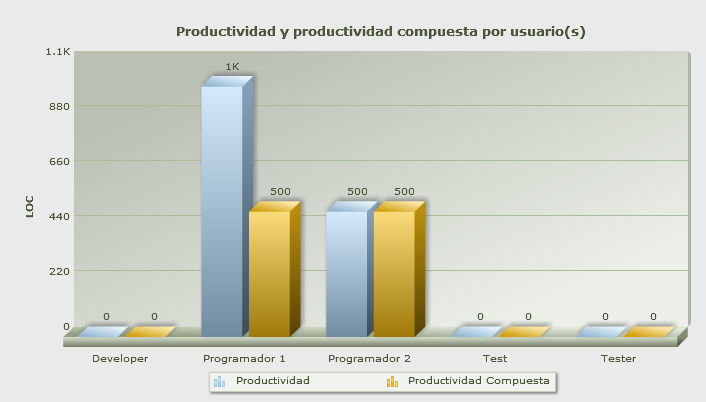
\includegraphics[scale=0.9]{images/SSreportes2BM.png}
	\caption{Productividad Compuesta}
	\label{fig:SSreportes2BM}
\end{figure}

\subsubsection{ROI de Proyecto/Empresa}
\label{sec:ROIdeProyecto/Empresa}
\noindent
El ROI de Proyecto/Empresa es un reporte a nivel proyecto y organizaci�n. Este reporte realiza el c�lculo del ROI de las actividades de calidad realizadas en un proyecto, y compara el costo real del proyecto contra el costo que hubiera tenido si no se implementan las t�cnicas de calidad. Para realizar el c�lculo de lo que hubiera costado el proyecto se toma en cuenta la regla de que el esfuerzo para remover un defecto aumenta diez veces cada fase que permanece en el proyecto\cite{Lazic2009}. Las f�rmula utilizada para generar este reporte es la siguiente:

\begin{math}ROI = \frac{QF - QA}{QA}\end{math}

Donde:

\begin{itemize}
	\item ROI: Retorno de Inversi'on.
	\item QF: Costo de Correcci'on de Defectos.
	\item QA: Costo de las Actividades de Calidad.
\end{itemize}

La figura \ref{fig:SSreportes3BM} muestra un ejemplo de como se ve el reporte en el BM. Este reporte es muy �til para las organizaciones en el sentido que muestra una visi�n general de la efectividad de las t�cnicas de calidad del proyecto, en otras palabras, eval�a las t�cnicas en t�rminos de tiempo y dinero.

\begin{figure}[h]
	\centering
		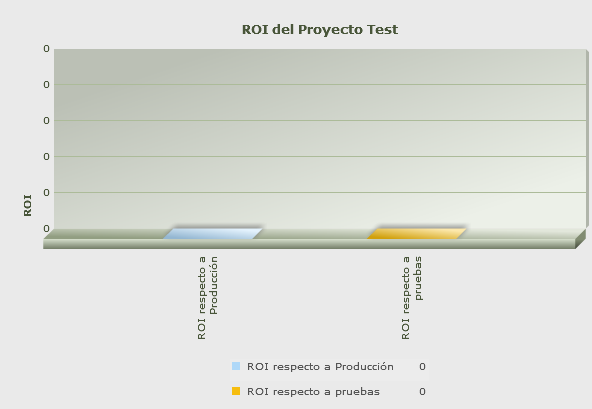
\includegraphics[scale=0.9]{images/SSreportes3BM.png}
	\caption{ROI de Proyecto u Organizaci'on}
	\label{fig:SSreportes3BM}
\end{figure}

\subsubsection{ROI de T'ecnicas de Detecci'on}
\label{sec:ROIdeTecnicasdeDeteccion}
\noindent
El ROI de T'ecnicas de Detecci'on es un reporte a nivel proyecto y organizaci'on. Es similar al reporte de ROI de Proyecto/Empresa en el sentido que pone las t'ecnicas de calidad en t'erminos de tiempo y dinero, pero lo hace de forma individual. En vez de calcular el ROI total del proyecto, lo hace por separado con cada t'ecnica. Este reporte nos permite hacer una evaluaci'on m'as profunda del ROI y evaluar que t'ecnicas son m'as efectivas y convenientes de implementar que otras.

\subsubsection{CoQ vs CNQ}
\label{sec:CoQvsCNQ}
\noindent
El CoQ vs CNQ es un reporte a nivel proyecto y organizaci'on. Este hace una comparaci'on entre el costo de conformidad y el costo de la no conformidad (ver secci'on \ref{sec:costodelacalidaddesoftware}). Las organizaciones de software deben intentar que exista un balance entre estos costos, visto de otra forma, el CoQ y el CNQ deben de ser similares. La figura \ref{fig:SSreportes4BM} nos muestra el reporte dentro del BM.

\begin{figure}[h]
	\centering
		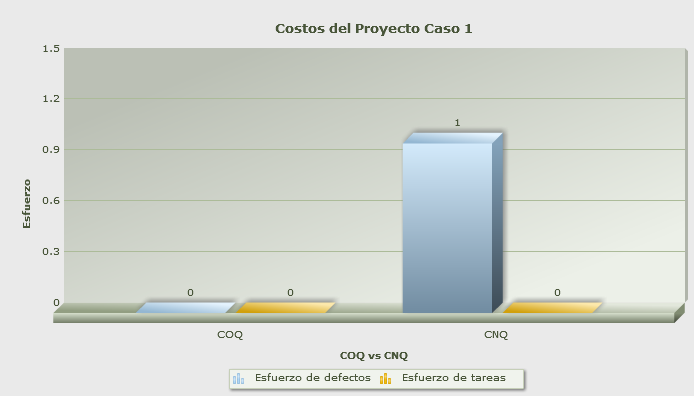
\includegraphics[scale=0.9]{images/SSreportes4BM.png}
	\caption{CoQ vs CNQ}
	\label{fig:SSreportes4BM}
\end{figure}

\subsubsection{Yield por T'ecnica de Detecci'on}
\label{sec:YieldporTecnicadeDeteccion}
\noindent
El Yield por T'ecnica de Detecci'on es un reporte a nivel proyecto y organizaci'on. Indica la eficiencia de cada t'ecnica de detecci'on en la detecci'on de defectos. En otras palabras indica que porcentaje del total de defectos detect'o dicha t'ecnica.

\subsubsection{N'umero de Defectos por T'ecnica de Detecci'on}
\label{sec:NumerodeDefectosporTecnicadeDeteccion}
\noindent
El n'umero de defectos por t'ecnica de detecci'on es un reporte a nivel proyecto y organizaci'on. Indica el n'umero de defectos detectados por cada t'ecnica de detecci'on de defectos. 

\subsubsection{Esfuerzo por T'ecnica de Detecci'on}
\label{sec:EsfuerzoporTecnicadeDeteccion}
\noindent
El esfuerzo por t'ecnica de detecci'on es un reporte a nivel proyecto y organizaci'on. Indica el esfuerzo que se tom'o en cada t'ecnica de detecci'on de defectos.

\subsubsection{Eficiencia por T'ecnica de Detecci'on}
\label{sec:EficienciaporTecnicadeDeteccion}
\noindent
La eficiencia por t'ecnica de detecci'on es un reporte a nivel proyecto y organizaci'on. Surge al conjuntar el reporte de N'umero de Defectos por T'ecnica de Detecci'on y el Esfuerzo por T'ecnica de Detecci'on. Indica cuantos defectos detecta por hora cada t'ecnica de detecci'on. Se calcula con la siguiente f'ormula:

\begin{math}E = \frac{DT}{ET}\end{math}

Donde:

\begin{itemize}
	\item E: Eficiencia por T'ecnica de Revisi'on.
	\item DT: Defectos Detectatados por T'ecnica de Revisi'on.
	\item ET: Esfuerzo Total en T'ecnica de Revisi'on.
\end{itemize}

\subsubsection{Raz'on de Revisi'on por T'ecnica de Detecci'on}
\label{sec:RazonporTecnicadeDeteccion}
\noindent
La raz'on de revisi'on por t'ecnica de detecci'on es un reporte a nivel proyecto y organizaci'on. Indica la velocidad a la que se realizan las distintas t'ecnicas de detecci'on de defectos. Para actividades de revisi'on de c'odigo se recomienda una velocidad de 300-500 LOC por hora\cite{SmartBear}. Esta velocidad nos permite un enfoque suficiente a cada l'inea sin caer en una p'erdida de tiempo. Una estrategia para aumentar el Yield de las revisiones de c'odigo puede ser realizar las revisiones de c'odigo al ritmo mencionado anteriormente. La f'ormula que se utiliza para calcular la raz'on de revisi'on es la siguiente:

\begin{math}R = \frac{S}{T}\end{math}

Donde:

\begin{itemize}
	\item R: Raz'on de Revisi'on.
	\item S: Tama'no Total del Producto Revisado.
	\item T: Tiempo Total de la Revisi'on.
\end{itemize}

\subsubsection{Densidad de Defectos}
\label{sec:DensidaddeDefectos}
\noindent
La densidad de defectos es un reporte a nivel usuario, proyecto y organizaci'on. La densidad de defectos es el n'umero de defectos encontrados en un proyecto por cada KLOC. La figura \ref{fig:densidaddefectoscmmitsp} presenta la densidad de defectos para organizaciones con niveles de CMMI 1, 2, 3, 4,5 y organizaciones con TSP. Con esta gr'afica podemos hacer una evaluaci'on del nivel de calidad del proyecto.

\begin{figure}[h]
	\centering
		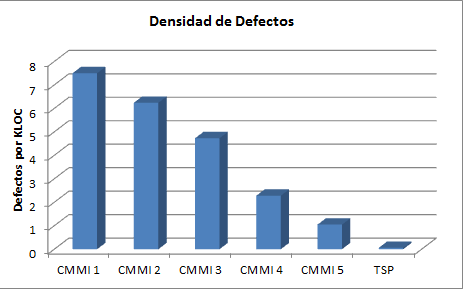
\includegraphics[scale=0.9]{images/DensidadDefectos.png}
	\caption{Densidad de Defectos por Nivel de CMMI y TSP}
	\label{fig:densidaddefectoscmmitsp}
\end{figure}

Este reporte se calcula con la siguiente f'ormula:

\begin{math}DD = 1000*\frac{D}{S}\end{math}

Donde:

\begin{itemize}
	\item DD: Densidad de Defectos.
	\item D: N'umero Total de Defectos.
	\item S: Tama'no del Producto.
\end{itemize}

\subsubsection{N'umero de Defectos por Tipo}
\label{sec:NumerodeDefectosporTipo}
\noindent
El n'umero de defectos por tipo es un reporte a nivel usuario, proyecto y organizaci'on. Indica el n'umero de defectos clasificados por tipo que se inyectaron. Con este reporte se pueden plantear estrategias para detectar y evitar cometer los defectos m'as comunes. Por ejemplo se pueden actualizar las plantillas de calidad para detectar determinado tipo de defecto.

\subsubsection{Defectos Inyectados y Removidos por Fase}
\label{sec:DefectosInyectadosyRemovidosporFase}
\noindent
El reporte de defectos inyectados y removidos por fase es a nivel usuario, proyecto y organizaci'on. Indica el n'umero de defectos que se inyectan y se remueven en cada fase.

\clearpage